\section{Meditation on the Immaculate Conception}

\begin{wrapfigure}{rt}{.35\textwidth}
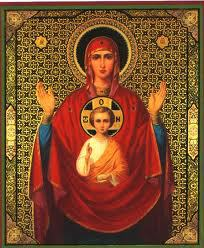
\includegraphics[scale=.6]{a20221208MeditationontheImmaculateConception-img001.jpg} 
\end{wrapfigure}

\begin{quotationx}
One can also say that the incarnated human being is the product of two heredities — horizontal
heredity and vertical heredity, the latter being the imprint of the individuality from above and the former being the
imprint of the ancestors here below. This seeks to express that he is the product of two imitations
— horizontal and vertical, i.e., that in order to become what he is he owes it to imitation of his
ancestors from the past and to that of himself above. In the last analysis, therefore, it is a matter on the one hand
of horizontal heredity going back to the archetype or terrestrial heredity, i.e. Adam, and on the other hand of
vertical heredity rising up to the Father who is heaven, i.e., God. This is why it is so important to allow light from
the dogma of the \textbf{immaculate conception} to convince us of its truth, for what is at stake is the line of
vertical heredity — “God-man heredity”. 
\flright{\textsc{Valentin Tomberg}}

The Father gave her his Son, the Son came down into her virginal womb to become her child; in her the Holy Spirit
miraculously fashioned the body of Jesus and made her soul his own dwelling place, penetrating her whole being such an
ineffable manner that the expression “Spouse of the Holy Spirit” is far from adequate to express the life of the Spirit
in her and through her. In Jesus there are two natures, divine and human, but one single Person who is God; here on the
contrary we have two natures and two persons, the Holy Spirit and the Immaculata, but united in a union that defies all
human expression. \flright{\textsc{St Maximilian Kolbe}}

For the Word generated by the Father is understood by the one in whom it is received perfectly — by
that person who is the Immaculate Conception. \flright{\textsc{St Maximilian Kolbe}}

By the power of the Holy Spirit the Word became incarnate from the Virgin Mary. \flright{\itshape Nicene Creed} 

\end{quotationx}

Just as Eve was the genetic equivalent to Adam, apart from the X chromosome, so likewise is the New Adam the genetic
equivalent to the New Eve. In our time, given our knowledge of biology and genetics, the possibility of a virginal
conception is no longer inconceivable.

So Jesus, the New Adam, is the genetic image of his Mother, Mary, the New Eve. Moreover, while the body of Jesus was in
Mary's womb, her soul was, in Kolbe's words, the dwelling place of the Holy
Spirit. As we saw in Letter II on the High Priestess, the Holy Spirit can be reflected only in the completely
unperturbed soul, a soul protected from sin. That is Mary, who understood the Spirit perfectly.

As Tomberg points out, we are under the law of horizontal heredity, in imitation of our ancestors, going back to Adam.
This prepares the biological and social environment in which the individuality can incarnate. Hence, Jesus appears at a
specific time and place, to the mother prepared to receive him.

While Mary was “full of grace” from the beginning, we are likewise called to be full of grace; this is \emph{theosis}.
This is confirmed in Mary as the Queen of Heaven. For us, it is something to be achieved. For that, she is our model.

Jesus has two natures, divine and human, in one Person. We, through \emph{theosis}, can have a divine as well as a human
nature. However, we retain our own Person, so this union of the human with the divine requires two persons. By
purifying our own soul, the Holy Spirit can become more fully reflected in our own consciousness. Then the Logos is
born in us, too, and we put on our true Self:

\begin{quotationx}
And I live, now not I; but Christ liveth in me. And that I live now in the flesh: I live in the faith of the Son of God,
who loved me, and delivered himself for me. \flright{\itshape Galatians 2:20}
\end{quotationx}

\flright{\itshape Posted on 2022-12-08 by Cologero}

\begin{center}* * *\end{center}

\begin{footnotesize}
\texttt{DEWnada on 2022-12-08 at 16:36 said: }

The Theotokos can be considered the Pneumatophoric Hypostasis according to Bulgakov. If we apply
Tomberg's Luminous Holy Trinity model with Bulgakov's Sophiology we then get:
Mary, the World Soul / Holy Soul, consort of the Holy Spirit \& Pneumatophoric Hypostasis; Bat Kol / Shabbat HaMalka,
Daughter of God, consort of the Son of God / the Logos \& the Logophoric Hypostasis; and Elat / Al-Kat, the Divine
Mother consort of the Divine Father El and the Mysteriophoric Hypostasis. Trino-Sophia is here seen as the transcendent
uncreated Sophia Mother, the mediating unbegotten Sophia Crone-Daughter, and the immanent created Sophia
Virgin-Immaculata. I made up the Logophoric and Mysteriophoric Hypostases terms and welcome better conceptual
designations. Critique and amplify. Sat Naam

\end{footnotesize}

